\begin{pastexam}[label={px:gk3-106-ds-02}]{高考三級資訊處理 106 年 第二題}
（申論；20 分）

遊樂園設計公司正在設計新的遊樂園，遊樂園將有 9 個遊樂設施，設施名稱暫定為 A, B, C, D, E, F, G, H, I。
遊樂設施之間將透過不盡相同距離但極具特色的商店街相連。給定遊樂園的初步規劃如表一，表內數字為兩遊樂
設施之間商店街道之預計長度（每條街道長度皆不同）。若無數字則代表兩遊樂設施之間沒有商店街道之規劃。
設計公司將依不同考量來決定實際建置那些商店街道。
\begin{center}
表一\\[2pt]
\small
\begin{tabular}{|c|*{9}{c|}}
\hline
 & A & B & C & D & E & F & G & H & I \\ \hline
A &    & 18 &    & 5  & 13 & 1  &    &    &    \\ \hline
B & 18 &    & 9  &    & 10 & 16 &    &    & 8  \\ \hline
C &    & 9  &    &    & 11 &    & 7  & 12 & 3  \\ \hline
D & 5  &    &    &    & 17 &    & 19 &    &    \\ \hline
E & 13 & 10 & 11 & 17 &    &    & 2  &    &    \\ \hline
F & 1  & 16 &    &    &    &    &    & 14 & 15 \\ \hline
G &    &    & 7  & 19 & 2  &    &    & 4  &    \\ \hline
H &    &    & 12 &    &    & 14 & 4  &    & 6  \\ \hline
I &    & 8  & 3  &    &    & 15 &    & 6  &    \\ \hline
\end{tabular}
\end{center}
\begin{itemize}[leftmargin=2.2em]
\item[㈠] 若要節省開發預算，在可到達所有遊樂設施的前提下，所建置的商店街道總長度需越短越好，請問可以用
那一個演算法來選擇應建置的街道？請給演算法名稱並簡單說明該演算法特性。（5 分）
\item[㈡] 請計算符合上述㈠小題條件下，所應建置的商店街道總長度，並由小到大列舉所有應該建置街道的長度。
（10 分）
\item[㈢] 但若要規劃一條路徑，使得遊客可以從任一遊樂設施開始玩，且只要依照該路徑行走，就可以玩遍 9 項
遊樂設施並回到起始的遊樂設施，遊客所需走過的商店街道總長度需越短越好且每項遊樂設施只能到達一次。
請問此問題最適合用下列那一種演算法來幫忙找到所應開發的街道：尤拉迴路（Euler Cycle），漢密爾頓迴路
（Hamiltonian Cycle），旅行商人問題（Traveling Sales Man Problem），最短路徑（例如 Dijkstra 演算法），
任兩點最短距離（例如弗洛伊德(Floyd-Warshall)演算法）？（5 分）
\end{itemize}
\end{pastexam}

\begin{pastsoln}
答案：㈠ 最小生成樹演算法，例如 Kruskal（或 Prim）；㈡ 總長度 $42$，各街道長度
$1, 2, 3, 4, 5, 6, 8, 13$；㈢ 旅行商人問題。 ㈢ 屬第~28~章，整題以最小生成樹為主，放在第~24~章。

把設施當頂點、商店街當邊、長度當權重，表一是一張 $9$ 個頂點、$19$ 條邊的無向加權圖（表是對稱的，
每條邊在表裡出現兩次）。 依權重列出所有邊：
\begin{center}
\small
\setlength{\tabcolsep}{3.5pt}
\begin{tabular}{l*{19}{c}}
\toprule
權重 & 1 & 2 & 3 & 4 & 5 & 6 & 7 & 8 & 9 & 10 & 11 & 12 & 13 & 14 & 15 & 16 & 17 & 18 & 19 \\
\midrule
邊 & AF & EG & CI & GH & AD & HI & CG & BI & BC & BE & CE & CH & AE & FH & FI & BF & DE & AB & DG \\
\bottomrule
\end{tabular}
\end{center}

\textbf{㈠} 「每個設施都到得了、總長度最短」就是求這張圖的\textbf{最小生成樹}（minimum spanning tree）：
連通所有頂點、沒有環（有環就能拿掉環上一條邊而仍然連通、長度更短），總權重最小。 可以用
\textbf{Kruskal 演算法}（資結書第~24.2~節）：
\begin{itemize}
\item 貪心法：把邊依權重由小到大排序，依序考慮，加入後不會形成環就加入，否則丟掉；加滿 $n - 1$ 條邊就停。
\item 用互斥集合（union-find）判斷兩端點是否已經連通，時間 $O(|E| \log |E|)$，主要花在排序。
\item 正確性來自切割性質：每次加入的邊是跨越某個切割的最輕邊，一定屬於某棵最小生成樹。 邊權都不同時
最小生成樹唯一。
\end{itemize}
也可以答 Prim 演算法（資結書第~24.3~節，從一個頂點開始，每次加入連到樹外最輕的邊）或 Sollin
（Bor\r{u}vka）演算法，結果相同。

\textbf{㈡} 用 Kruskal 逐邊處理：
\begin{center}
\small
\begin{tabular}{ccll}
\toprule
權重 & 邊 & 結果 & 加入後的集合（只列兩點以上的） \\
\midrule
1 & A--F & 加入 & $\{A, F\}$ \\
2 & E--G & 加入 & $\{A, F\}$, $\{E, G\}$ \\
3 & C--I & 加入 & $\{A, F\}$, $\{E, G\}$, $\{C, I\}$ \\
4 & G--H & 加入 & $\{A, F\}$, $\{E, G, H\}$, $\{C, I\}$ \\
5 & A--D & 加入 & $\{A, D, F\}$, $\{E, G, H\}$, $\{C, I\}$ \\
6 & H--I & 加入 & $\{A, D, F\}$, $\{C, E, G, H, I\}$ \\
7 & C--G & 跳過（成環 C--G--H--I） & \\
8 & B--I & 加入 & $\{A, D, F\}$, $\{B, C, E, G, H, I\}$ \\
9--12 & \multicolumn{3}{l}{B--C、B--E、C--E、C--H 都跳過（兩端已在同一集合）} \\
13 & A--E & 加入 & 全部 $9$ 個頂點 \\
\bottomrule
\end{tabular}
\end{center}
第 $13$ 的邊是第 $8$ 條（$= 9 - 1$），停止。 應建置的街道長度由小到大是
$\mathbf{1, 2, 3, 4, 5, 6, 8, 13}$，總長度 $1 + 2 + 3 + 4 + 5 + 6 + 8 + 13 = \mathbf{42}$。 長度都
不同，這棵最小生成樹是唯一的，用 Prim 從任何頂點開始也會得到同樣這 $8$ 條。
\begin{center}
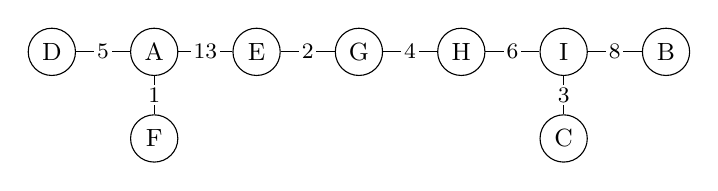
\begin{tikzpicture}[x=1.3cm,y=1.1cm,v/.style={circle,draw,minimum size=6mm,inner sep=0pt,font=\small},
    w/.style={fill=white,inner sep=1pt,font=\footnotesize}]
\node[v] (D) at (0,0) {D};
\node[v] (A) at (1,0) {A};
\node[v] (F) at (1,-1) {F};
\node[v] (E) at (2,0) {E};
\node[v] (G) at (3,0) {G};
\node[v] (H) at (4,0) {H};
\node[v] (I) at (5,0) {I};
\node[v] (C) at (5,-1) {C};
\node[v] (B) at (6,0) {B};
\draw (D)--node[w]{5}(A); \draw (A)--node[w]{1}(F); \draw (A)--node[w]{13}(E);
\draw (E)--node[w]{2}(G); \draw (G)--node[w]{4}(H); \draw (H)--node[w]{6}(I);
\draw (I)--node[w]{3}(C); \draw (I)--node[w]{8}(B);
\end{tikzpicture}
\end{center}

\textbf{㈢} \textbf{旅行商人問題}（TSP）。 「從某個設施出發、每個設施恰好到一次、最後回到起點」是
漢密爾頓迴路；再要求「總長度越短越好」，就是在所有漢密爾頓迴路裡找最短的，也就是旅行商人問題
（資結書第~28~章）。 其他選項：
\begin{itemize}
\item 尤拉迴路：每條\textbf{街道}恰好走一次，不是每個設施一次，不合題意。
\item 漢密爾頓迴路：只問「有沒有」這樣的迴路，不管長度，少了「最短」這個條件。
\item Dijkstra、Floyd--Warshall：求兩點之間的最短路徑，不要求經過所有設施、也不要求回到起點。
\end{itemize}
旅行商人問題是 NP 困難，沒有已知的多項式時間演算法；$9$ 個設施可以用動態規劃（$O(n^2 2^n)$）或分支
限界（資結書第~20~章）精確求解。 以這張圖為例，最短的環遊是 A--D--E--G--H--I--C--B--F--A，長度
$5 + 17 + 2 + 4 + 6 + 3 + 9 + 16 + 1 = 63$（題目沒有要求算出來）。
\end{pastsoln}
